\documentclass[aps,twocolumn,secnumarabic,amsmath,amssymb,nofootinbib]{revtex4-1}

% Documentclass Options
    % aps, prl stand for American Physical Society and Physical Review Letters respectively
    % twocolumn permits two columns, of course
    % nobalancelastpage doesn't attempt to equalize the lengths of the two columns on the last page
        % as might be desired in a journal where articles follow one another closely
    % amsmath and amssymb are necessary for the subequations environment among others
    % secnumarabic identifies sections by number to aid electronic review and commentary.
    % nofootinbib forces footnotes to occur on the page where they are first referenced
        % and not in the bibliography
    % REVTeX 4 is a set of macro packages designed to be used with LaTeX 2e.
        % REVTeX is well-suited for preparing manuscripts for submission to APS journals.
%\usepackage{cite}
\usepackage{lgrind}        % convert program listings to a form includable in a LaTeX document
\usepackage{chapterbib}    % allows a bibliography for each chapter (each labguide has it's own)
\usepackage{color}         % produces boxes or entire pages with colored backgrounds
\usepackage{graphics}      % standard graphics specifications
\usepackage[pdftex]{graphicx}      % alternative graphics specifications
\usepackage{longtable}     % helps with long table options
\usepackage{epsf}          % old package handles encapsulated post script issues
\usepackage{bm}            % special 'bold-math' package
%\usepackage{asymptote}     % For typesetting of mathematical illustrations
\usepackage{thumbpdf}
\usepackage{changepage}   % for the adjustwidth environment
\usepackage{placeins} % for the \floatBarriar command
\usepackage{enumitem} % for changing bullet in lists
\usepackage[colorlinks=true]{hyperref}  % this package should be added after all others
                                        % use as follows: \url{http://www.usm.maine.edu/~pauln/MainSite/PHY240.html}



\begin{document}

\title{Measuring the charge-to-mass ratio using a pair of Helmholtz coils}
\author{Samuel Barton, Kate Hendrick, Jessamine Huang}
\email{samuel.barton@maine.edu}
\date{\today}
\affiliation{USM Departments of Physics, Computer Science, and Chemistry}

\begin{abstract}
In this experiment we attempted to measure the charge-to-mass ratio of an electron using a vacuum tube filled with mercury gas in conjunction with a pair of Helmholtz coils, and then compare our value with the accepted value. The value for $\frac{e}{m}$ we measured was $1.423\times10^{11} \pm 3.196\times10^{10} \frac{C}{kg}$ This value, even with our uncertainty, was below the accepted value for $\frac{e}{m}$ ($1.759\times10^{11} \pm 1.1\times10^3 \frac{C}{kg}$) ~\cite{value} by approximately 1\%. This was due in part to some unforseen error in our measurement which caused our uncertainty to be too small, and to an issue with the A/C voltage in our circuit causing our measurements to be too low. According to the original definition of this experiment by K. T. Bainbridge \cite{origin}, we were within the tolerance of 2\% of $\frac{e}{m}$; however, we were unsatisfied with our result.
\linebreak
\end{abstract}

\maketitle

%%%%%%%%%%%%%%%%%%%%%%%%%%%%%%%%%%%%%%%%%%%%%%%%%%%%
%
% Here is the main body of text
%
%%%%%%%%%%%%%%%%%%%%%%%%%%%%%%%%%%%%%%%%%%%%%%%%%%%%
\section{Introduction}

We are measuring the charge-to-mass ratio in an electron using a set of Helmholtz coils in conjunction with a vacuum tube filled with mercury gas. An alternating voltage accelerates a stream of electrons which are emitted into the vacuum tube and bent into a circle by the magnetic field generated by the coils. We then measure the alternating voltage, magnetic field at the center of the coils, and radii drawn out by the bent stream of electrons for a number of different voltages. With these data we can calculate the specific charge of an electron. Historically the specific charge of the electron is an important quantity because it was determined before either of $e$ or $m$ could be. J. J. Thomsen is credited with being the first to successfully measure this quantity in 1897 \cite{first_measurement}. Our experiment is a repetition of the one proposed by K.T Bainbridge in 1938 \cite{origin}, who based his version on the work done by A. Schuster \cite{schuster}, W. Kaufmann \cite{kaufmann}, and J. J Thomsen \cite{thomsen}.

\section{Theory}

The Lorentz force law states that the force on an electron passing through a magnetic field will be $\vec{F} = q(\vec{v} \times \vec{B})$. In our apparatus the beam of electrons travels at a right angle to the magnetic field generated by the Helmholtz coils, and so we can rewrite the above equation as $F = Bev$ where $B$ is the magnetic field, $e$ is the charge of an electron, and $v$ is the velocity of that electron. Now by Newton's second law we get that $\vec{F} = m\vec{a}$; however, since the force exerted by the magnetic field is always perpendicular to the velocity we know that we have centripetal acceleration and $F = \frac{mv^2}{r}$ where $r$ is the radius of the circle being drawn out by the stream of electrons (see figure \ref{fig:theory}). We can thus write $Bev = \frac{mv^2}{r}$. Now, since our electrons are being accelerated by a potential difference we know that their kinetic energy $T = \frac{1}{2}mv^2 = eV$ where $V$ is the accelerating voltage, in volts. Solving for $v$ gives $v = \sqrt{\frac{2eV}{m}}$, which when substituted back into our force equation gives, after some algebra, 
\begin{equation}
	\frac{e}{m} = \frac{2V}{B^2r^2}
	\label{eq:e_over_m}
\end{equation}
We will use this equation for our final calculation of $\frac{e}{m}$. 
\\\\

\begin{figure}[ht]
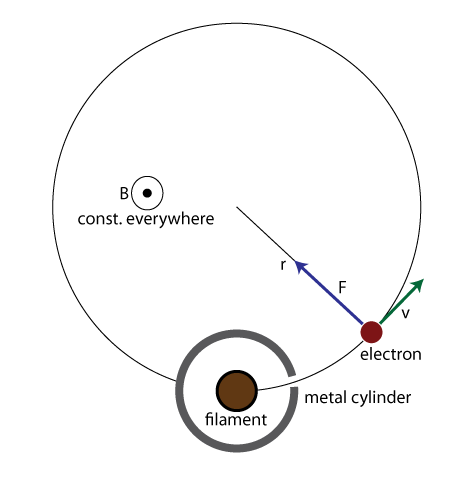
\includegraphics[width=9cm, keepaspectratio]{../images/e_over_m_theory.png}
\caption{Theoretical path of the electron.}
\label{fig:theory}
\end{figure}

To validate our measured value for $B$, we used the well-known equation for the magnetic field at the center of a pair of Helmholtz coils \cite{BHelmholtz}, \cite{detailed_b_helmholtz}
\begin{equation}
	B_{helmholtz} = \frac{8\mu_0NI}{a\sqrt{125}}
\label{eq:b_helmholtz}
\end{equation}
where $N$ is the number of turns in the Helmholtz coils, $I$ is the current through the coils, in amperes, and $a$ is the radius of the coils. Note that the radius of the electron beam can be changed by either the accelerating voltage, or the current through the Helmholtz coils.

\section{Apparatus}

Our apparatus consisted of a pair of Helmholtz coils, of radius $33 \pm 0.5cm$, with a vacuum tube in the center filled with mercury gas. Inside the spherical tube is a metal cylinder with an axial slit and a filament inside it. Creating a potential difference between the filament and the cylinder accelerates the electrons, some of which make it through the slit and form a beam which is then arced by the magnetic field from the Helmholtz coils. See figure \ref{fig:theory}. \\

\begin{figure}[htb]
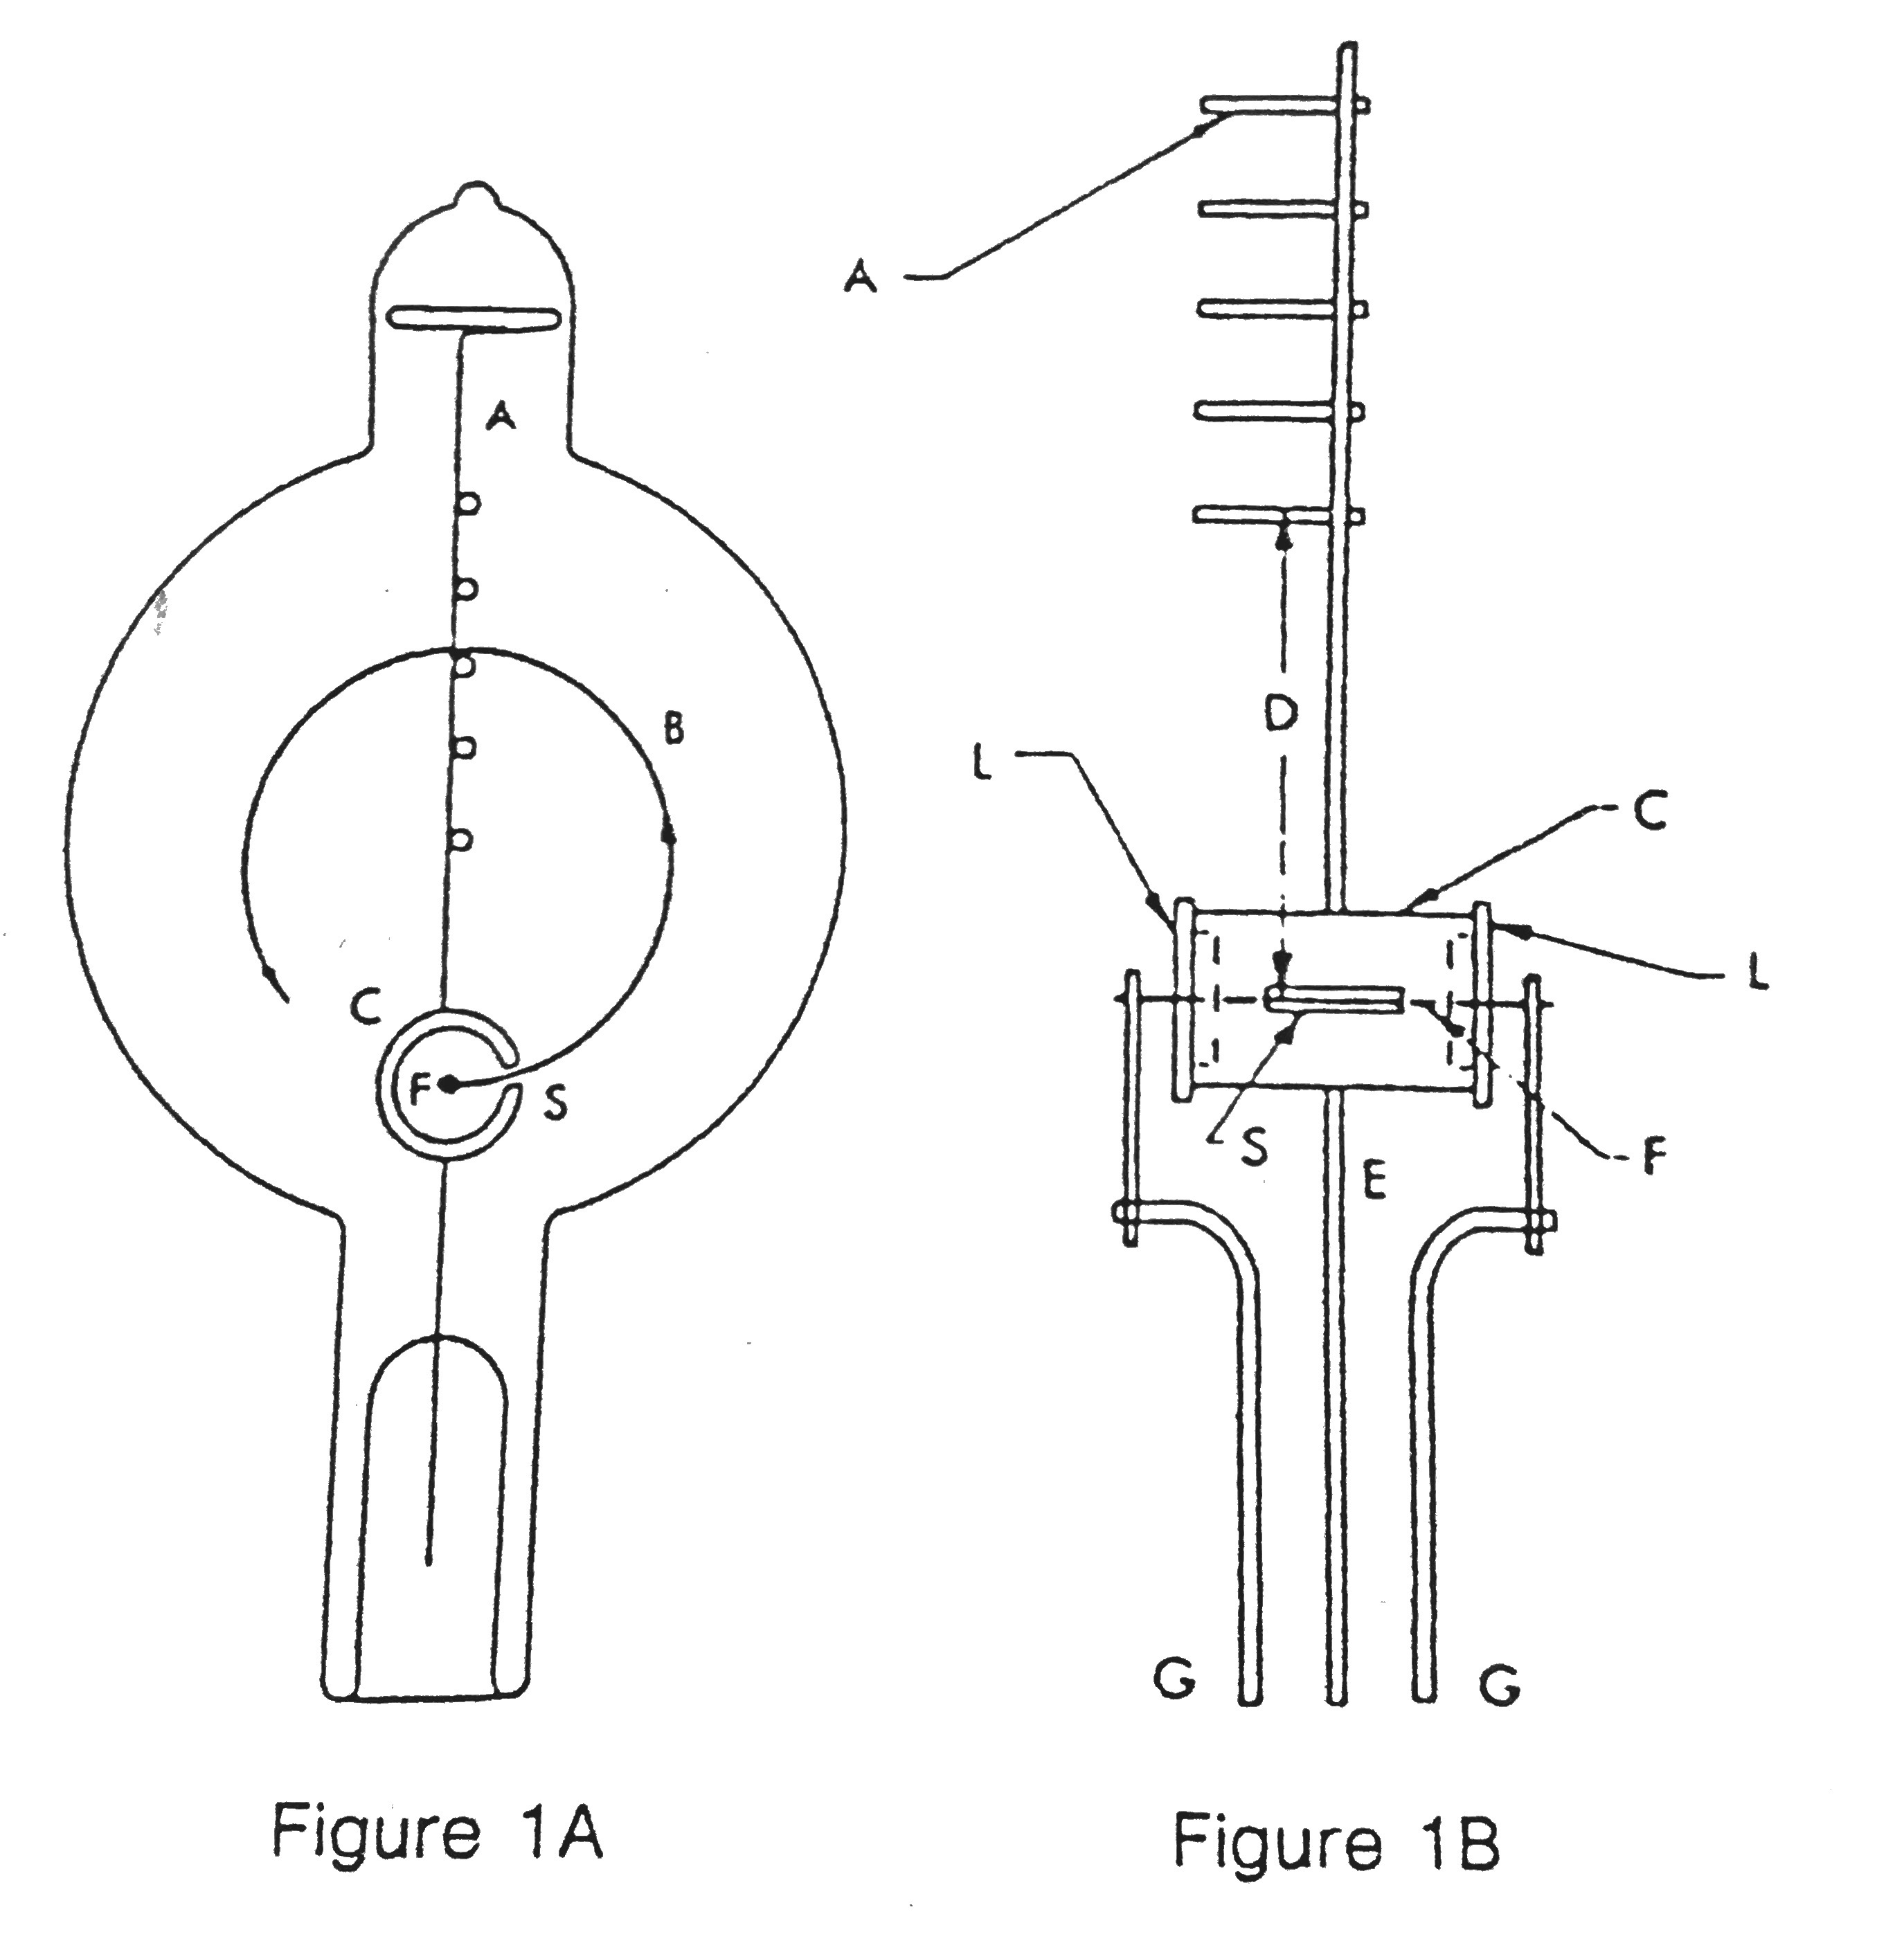
\includegraphics[width=7.5cm]{../images/e_over_m_apparatus.png}
\caption{This is a top down and side view of the vacuum tube assembly which sits in the center of the Helmholtz coils.}
\label{fig:apparatus}
\end{figure}

\begin{itemize}[label={}, nosep, noitemsep]
\item A\quad Five cross bars attached to staff wire.
\item B\quad Typical path of beam of electrons.
\item C\quad Cylindrical anode.
\item D\quad Distance from filament to far side of each of the cross bars.
\item E\quad Lead wire and support for anode.
\item F\quad Filament.
\item G\quad Lead wires and supports for filament.
\item L\quad Insulating plugs.
\item S\quad Slit in cylindrical anode. \\
\end{itemize}

We used a set of Vernier probes to measure the current going to the Helmholtz coils, the accelerating voltage, and the magnetic field at the center of the Helmholtz coils. These probes were attached to Logger Pro 3 via the USB interface, and were used to gather our data.\\

The entire assembly was mounted to a bracket and set on a table on casters so that it could be adjusted in each the of $\hat{R}$, $\hat{\theta}$, and $\hat{\phi}$ directions.

% Insert picture of the apparatus here

\section{Procedure}

Before we even thought about taking data we had to wire up the circuit which enables the apparatus to work in the first place, attach our probes into the circuit, and align the Helmholtz coils with the earths magnetic field by adjusting the apparatus in both the $\hat{\theta}$ and $\hat{\phi}$ directions until the axis of the apparatus shown in figure \ref{fig:apparatus} was aligned with magnetic north. To determine our alignment we used our cell phones with a number of compass apps and an app which tracked the direction of the earths magnetic field, and we also attempted to use some rather elderly physical compasses which were in the lab, but they were not consistent enough to be trusted.\\

We took seven sets of data consisting of five measurements of the magnetic field at the center of the coils, the accelerating voltage, and the current through the Helmholtz coils. We took one set of data for each radius $r$ we were given a value for (see figure \ref{fig:apparatus} and table ~\ref{tab:data}). These measurements were actually averages of five seconds of sampling the probes every $\frac{1}{20}th$ of a second. One team member adjusted the current and accelerating voltage, another validated their estimation of when the electron beam was at one of the known radii, and the last ran the Logger Pro interface. \\

Calibration of the magnetic field probe was done by putting it in the center of the coils when there was no field being generated, and shielding the probe with a cylinder of $\mu$ metal closed on one end. $\mu$ metal filters out magnetic fields, so when we set the zero point for that probe it was as close to zero as we could get. The voltage and current probes were set to zero when the circuit was completely off and the power sources were disconnected.

\section{Data Analysis}

% Insert a table of the averages from the iPython notebook
\begin{table}[ht]
\centering
\caption{One complete set of data for a particular accelerating voltage.}
\label{tab:data}
\begin{tabular}{lllll}
r (meters) & B (millitesla) & I (amperes) & V (volts)   &  \\ \hline
0.0575     & 0.35527826     & 2.06854256  & 29.85735903 &  \\
0.0515     & 0.3805583      & 2.28701536  & 29.85460338 &  \\
0.045      & 0.38050802     & 2.58383689  & 29.85532855 &  \\
0.039      & 0.38043454     & 2.97924697  & 29.8525729  &  \\
0.0325     & 0.38034365     & 3.41911728  & 29.85474841 &  \\
0.0575     & 0.34216211     & 2.00572106  & 27.7437871  & \\
\hline
\end{tabular}
\end{table}

We took the data from table \ref{tab:data}, along with the other thirty rows of data which aren't shown here (see Github repository \cite{github} for the rest of the data), and used Python to calculate $B_{helmholtz}$ using equation \ref{eq:b_helmholtz}. We compared $B_{helmholtz}$ to our measured value for the magnetic field at the center of the coils by graphing the measured current verses both of our values for the magnetic field.  This showed us that our probe was being saturated at around 2.3A, and thus the majority of our data could not be used (see figure \ref{fig:b_vals})

\begin{figure}[ht]
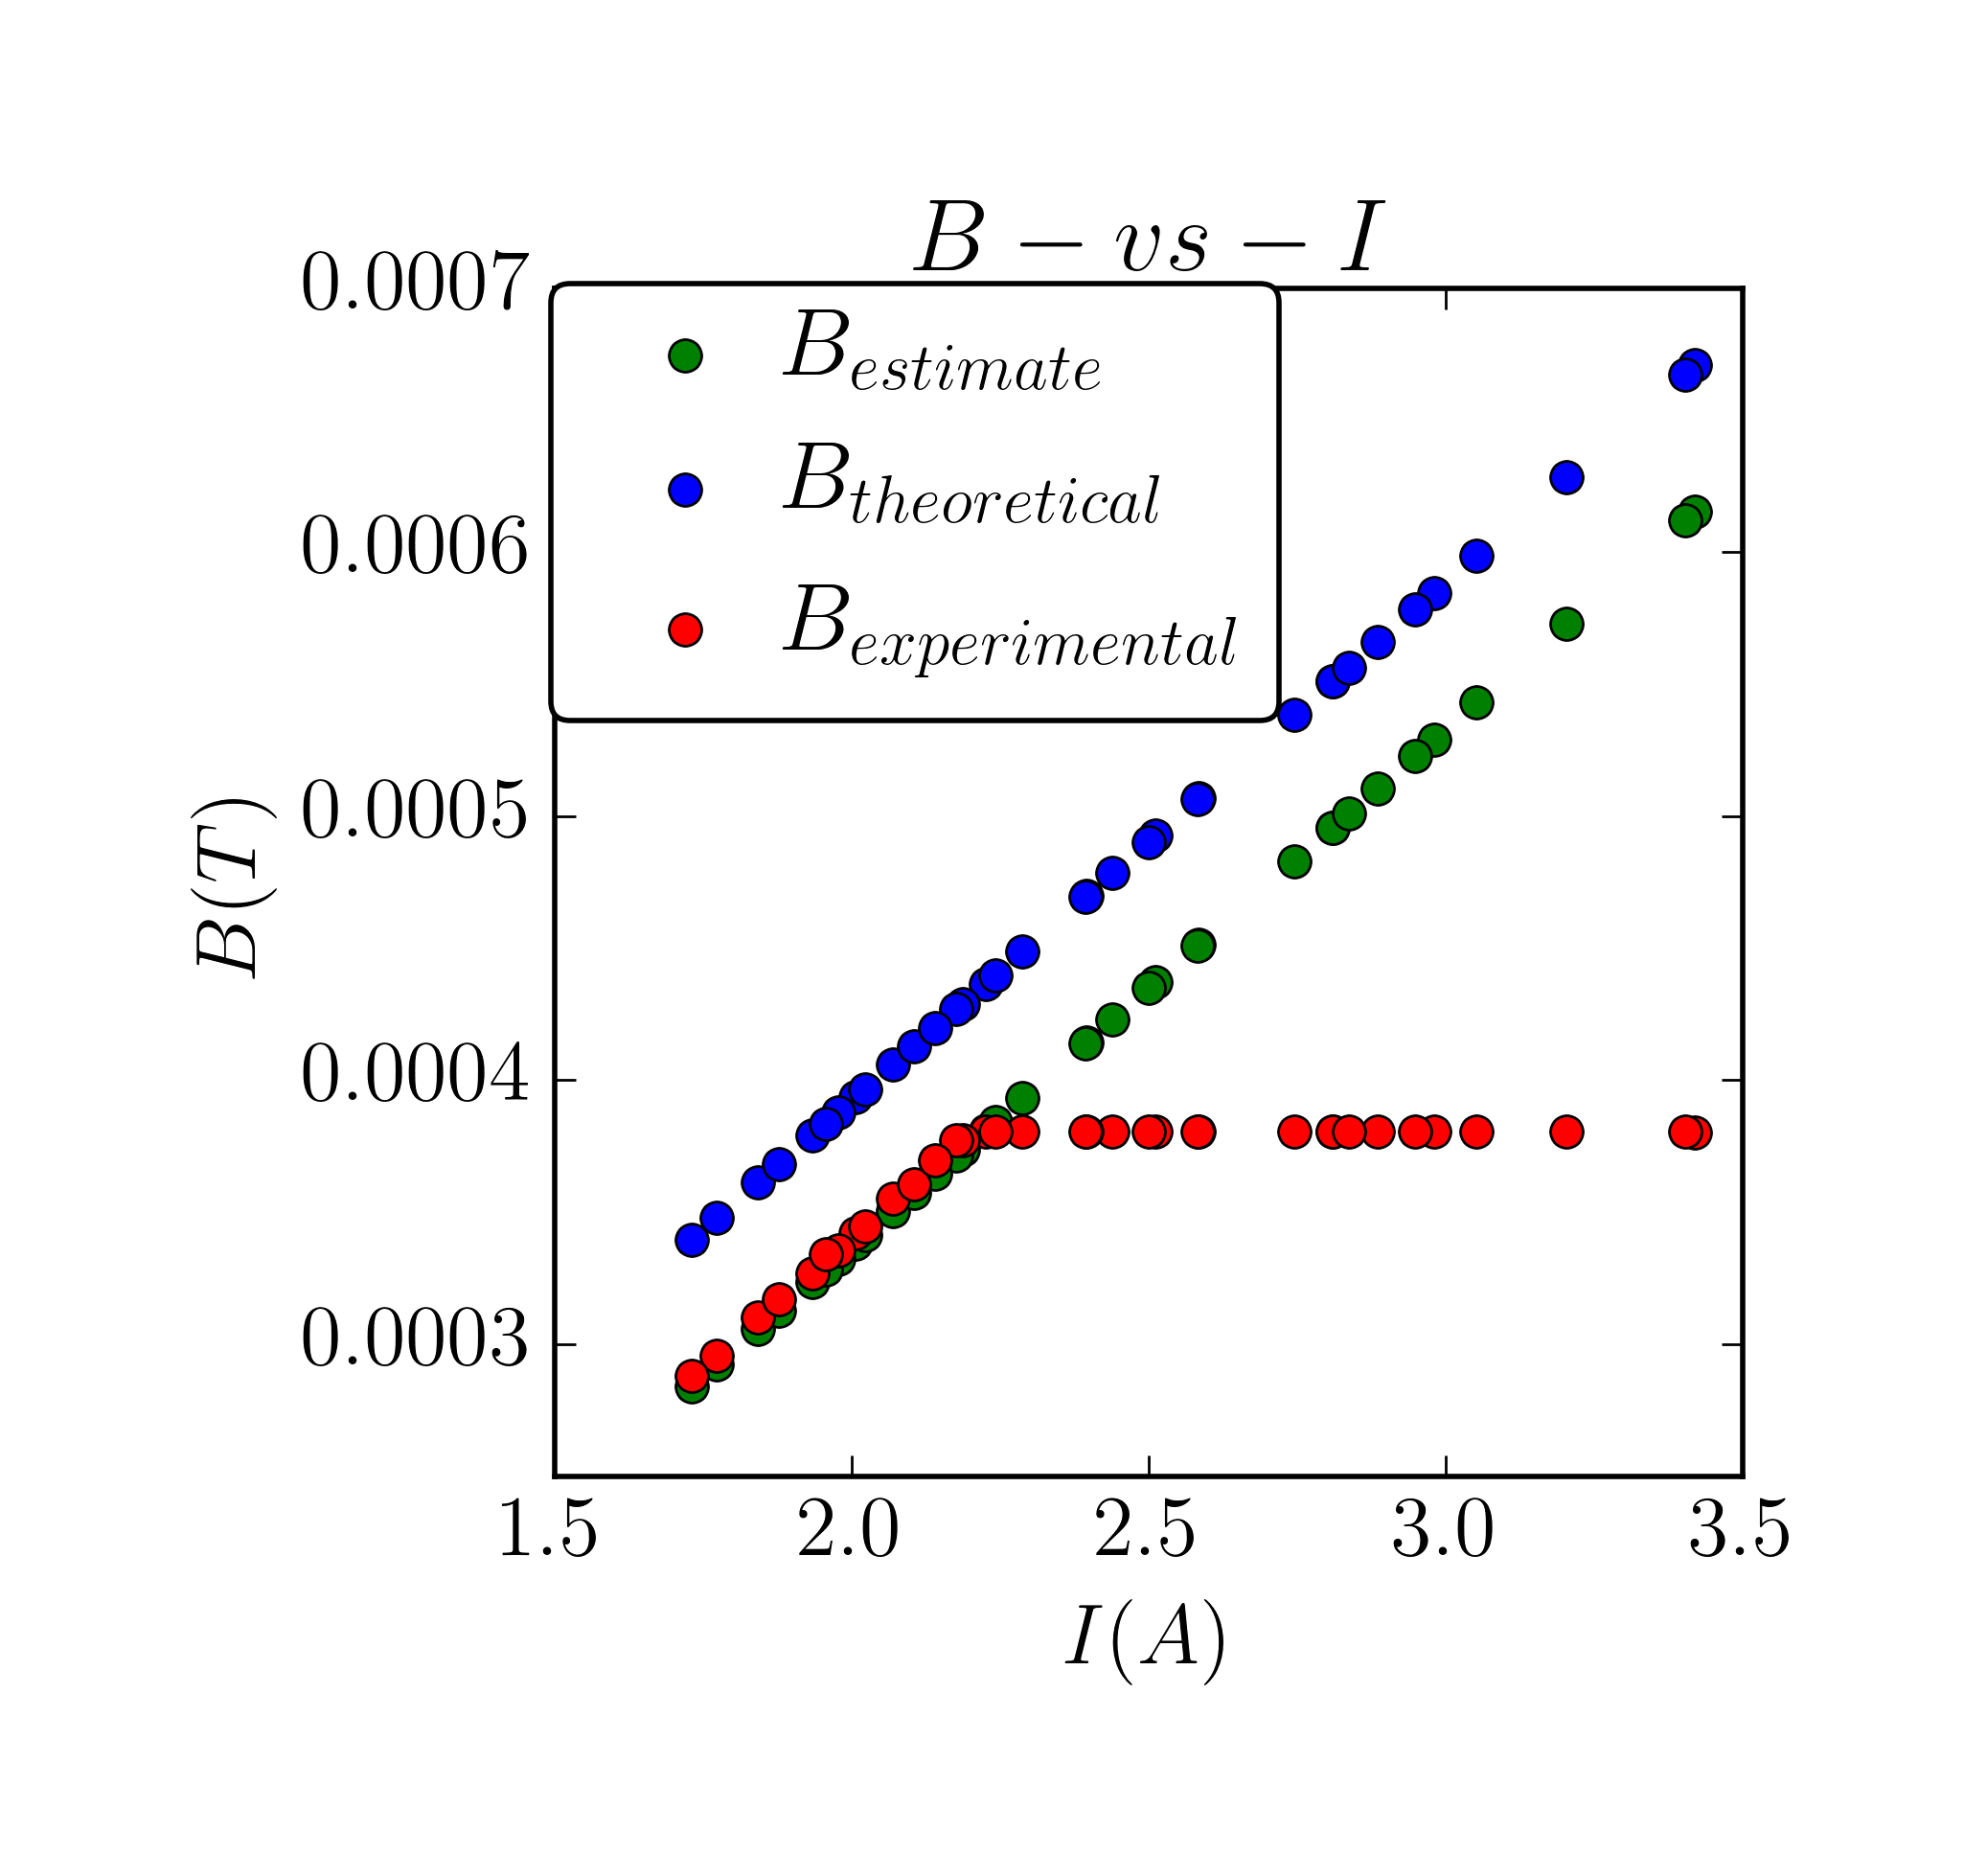
\includegraphics[width=9cm, keepaspectratio]{../images/comparing_b_5in.png}
\caption{Magnetic field values used in the experiment.}
\label{fig:b_vals}
\end{figure}

However all was not lost, as before the probe became saturated, there was a nearly constant difference between the probe's value for the magnetic field and $B_{helmholtz}$ as seen in figure \ref{fig:b_vals} by the parallelism between the blue and red lines before 2.3A. We calculated the mean difference between the two values for the magnetic field where they were parallel, and used that to extrapolate what the measured field should have been for all of the currents we measured. This is the green line in figure \ref{fig:b_vals}. We used our new value for the magnetic field, which we will call $B_{estimate}$ from here on out, in our calculation of $\frac{e}{m}$. \\

After getting $B_{estimate}$, we then put that back into equation \ref{eq:e_over_m} so that we could then plot $V-vs-\frac{1}{2}B_{estimate}^2r^2$ such that the slope of the best fit line of this plot would be our value for $\frac{e}{m}$. See figure \ref{fig:e_over_m} for the plot, error bars, best fit lines, slope information, and lower/upper bounds. See Jupiter Notebook in the \texttt{src} directory on Github \cite{github} for more information about the specific Python packages we used for calculating the best fit line and handling uncertainties.

\begin{figure*}[hb]
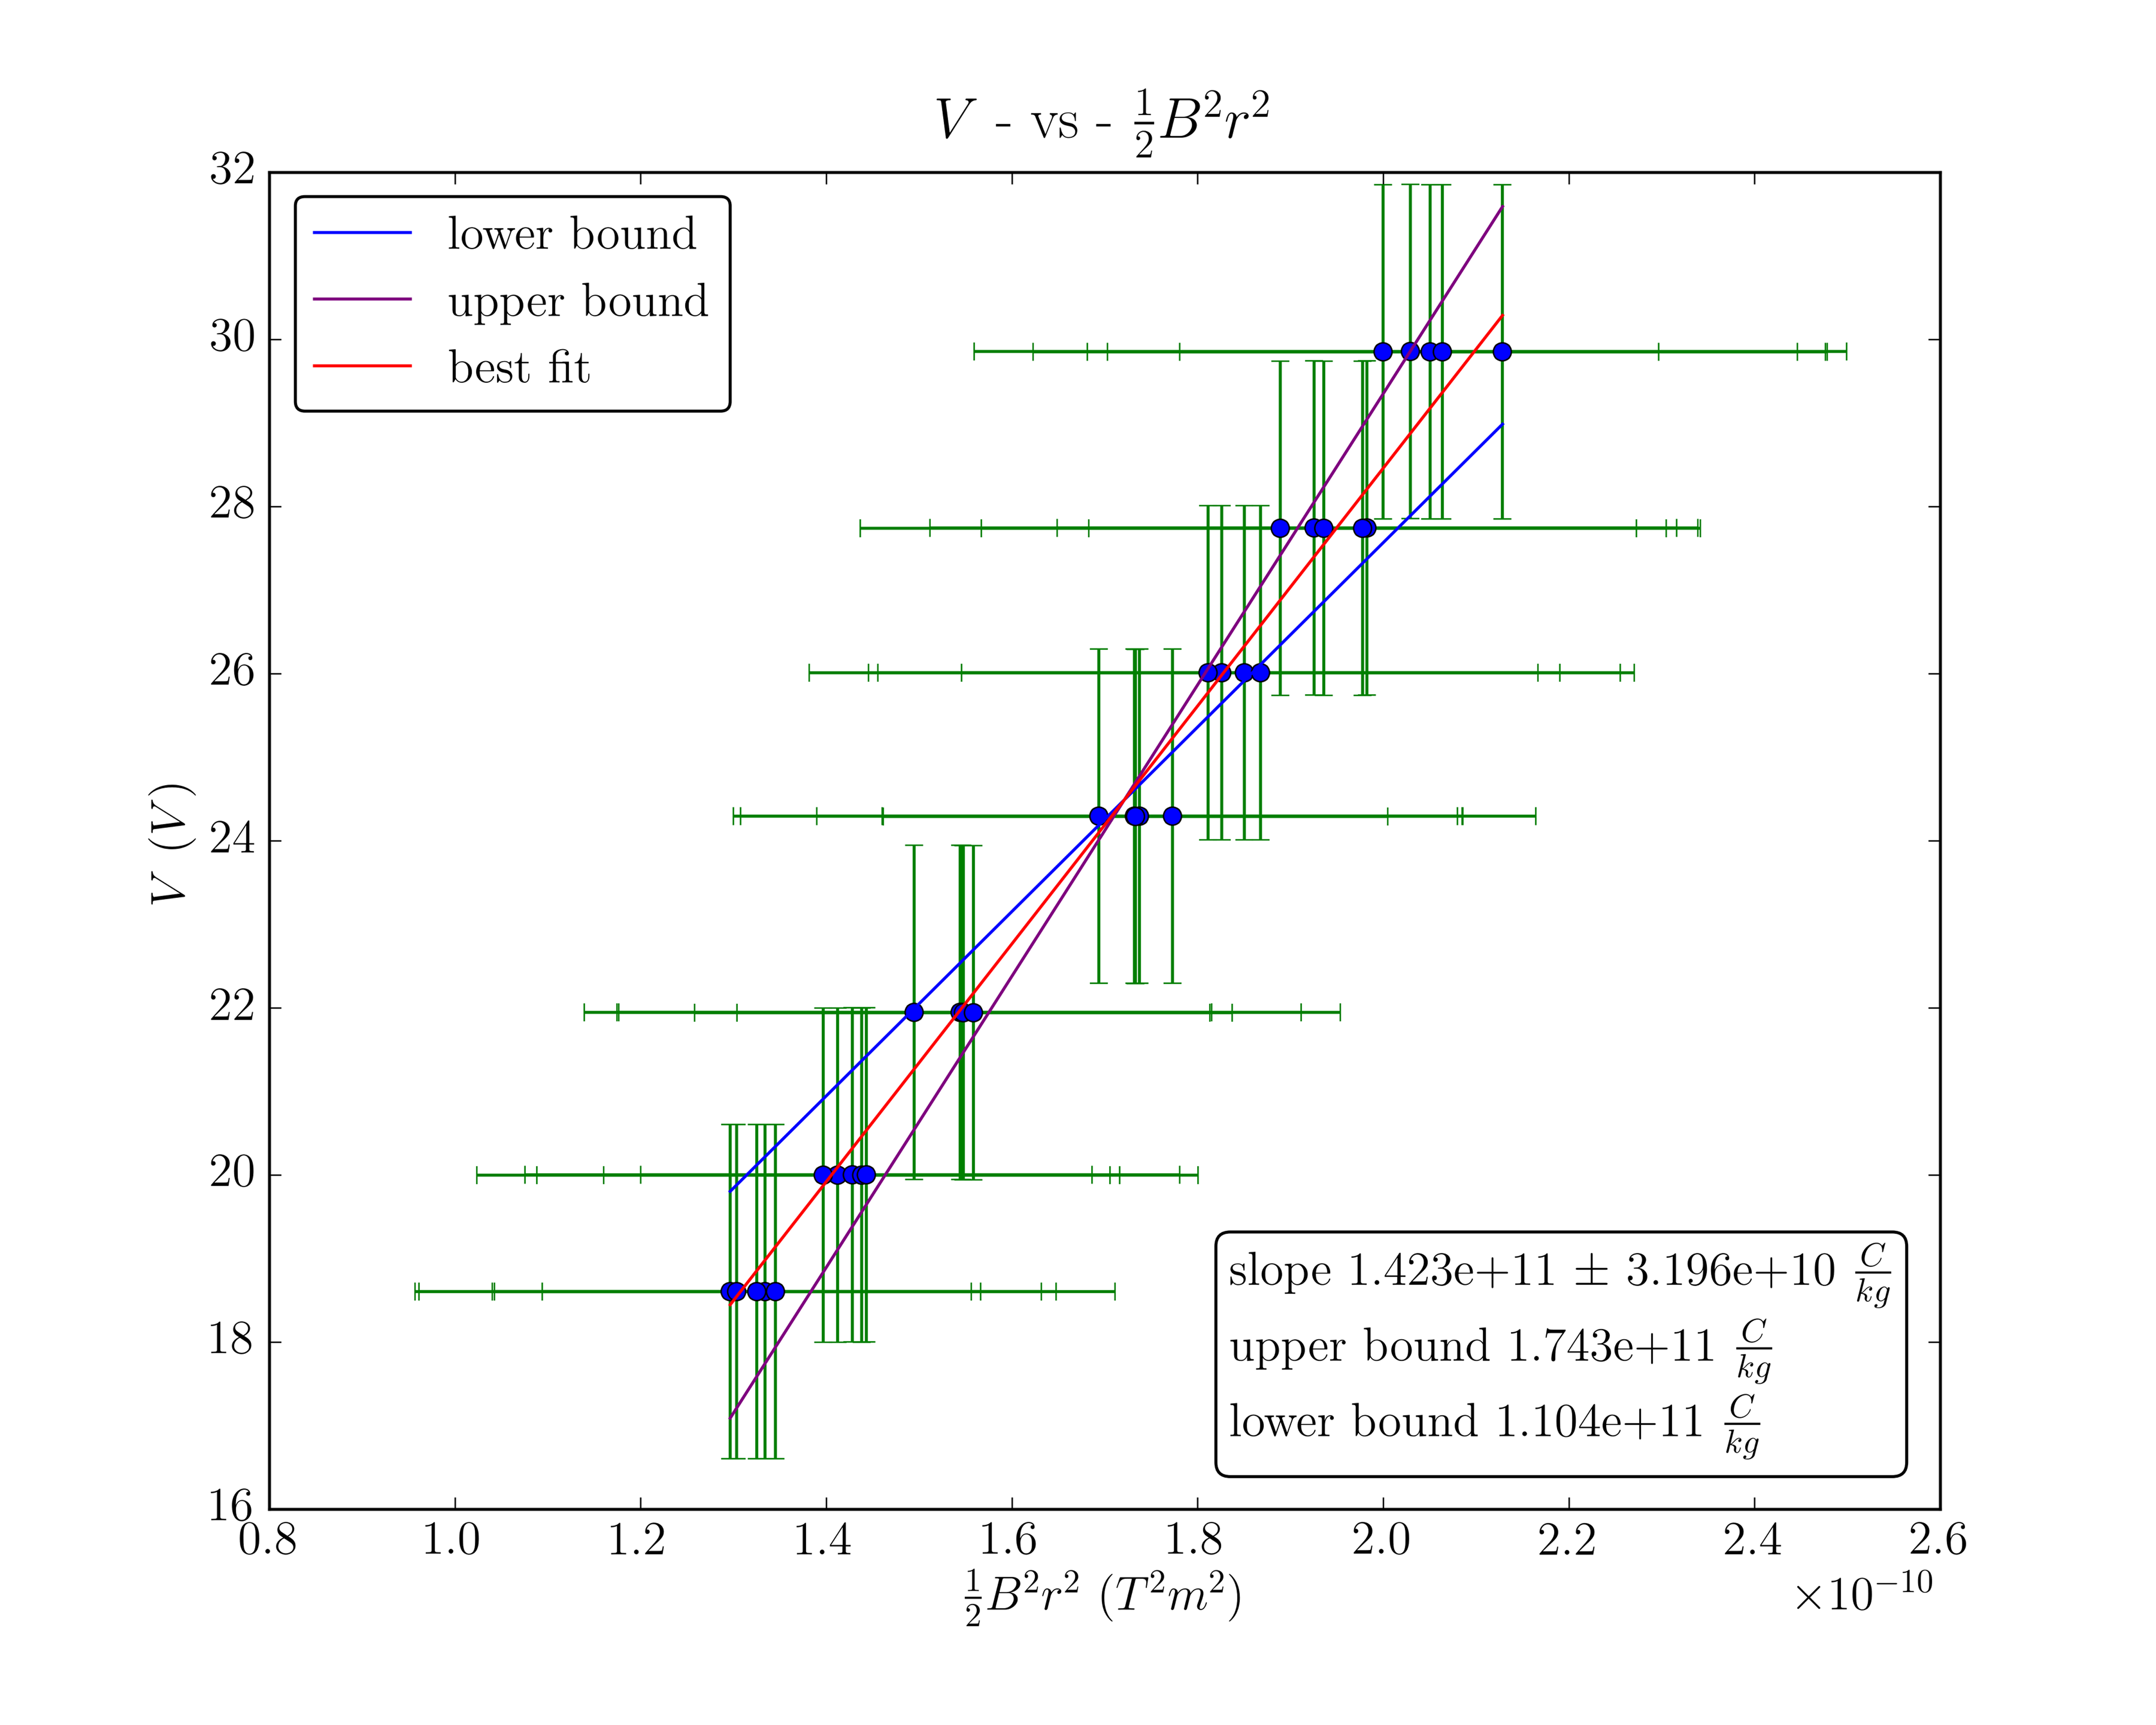
\includegraphics[width=\textwidth]{../images/e_over_m_8in.png}
\caption{The crucial part of this experiment. Our value for $\frac{e}{m}$ comes from the best fit line of this graph.}
\label{fig:e_over_m}
\end{figure*}

\section{Uncertainties and Error}

The following variables had uncertainties which we estimated based on difficulty of measurement, lack of confidence in given values, and tolerances in equipment:
\begin{itemize}[label={}, noitemsep]
	\item $V \pm 2$ volts
	\item $N \pm 1$ turn
	\item $r \pm 1$ millimeter
	\item $I \pm 0.2$ amperes
	\item $a \pm 0.5$ centimeters
\end{itemize}
Now $B_{estimate}$'s uncertainty changes as the current increases (see equation \ref{eq:b_helmholtz}), and its uncertainty is calculated from the uncertainties of $N$, $a$, and $I$. Below are the mean uncertainties for $B_{estimate}$
\begin{itemize}[label={}, noitemsep]
	\item $\delta I = \pm$ $7.847\times 10^{-6}$
	\item $\delta N = \pm$ $6.619 \times 10^{-6}$
	\item $\delta a = \pm$ $3.611 \times 10^{-8}$
\end{itemize}
When we calculate $\frac{e}{m}$, we get the uncertainties of $V$ and $r$ as well as those from $B_{estimate}$. This gives us a total uncertainty
\begin{align*}
	\delta(\frac{e}{m}) = \pm \ 3.196\times 10^{11} \frac{C}{kg}
\end{align*}
The relative contributions to the the total uncertainty of $\frac{e}{m}$ from each of our independent variables is:
\begin{itemize}[label={}, noitemsep]
	\item $\delta V = \pm \  2.426 \times 10^{10}$
	\item $\delta I = \pm \  5.569 \times 10^9$
	\item $\delta N = \pm \ 4.492 \times 10^9$
	\item $\delta a = \pm \ 2.450 \times 10^7$
	\item $\delta r = \pm \  6.488 \times 10^6$
\end{itemize}
The values for $\delta I$, $\delta N$, and $\delta a$ change so drastically because of the propagation of uncertainty which happens when they are fed into equation \ref{eq:e_over_m}. We see from the relative magnitudes of the uncertainties form $\frac{e}{m}$ that the source of greatest error was $V$, and unsurprisingly $r$ was the smallestl source of uncertainty. What this tells us is that we should have striven for greater precision in measuring both $V$ and $I$. The derivation of all of these uncertainties was done in Python (see Github repository \cite{github}).

\section{Results}

Our value for the specific charge, or charge-to-mass ratio of the electron is
\begin{align*}
	\frac{e}{m} = 1.423 \times 10^{11} \pm \ 3.196 \times 10^{10} \frac{C}{kg}
\end{align*}
Now, this value and uncertainty give the bounds for our measurement at $1.107 \times 10^{11}$ and $1.743 \times 10^{11} \frac{C}{kg}$. If we take the maximum value which our uncertainty allows, and compare it to the accepted value for $\frac{e}{m}$ of $1.759\times10^{11} \pm 1.1\times10^3 \frac{C}{kg}$ \cite{value} we get 
\begin{align*}
	\left(1 - \frac{1.743 \times 10^{11}}{1.759\times10^{11}}\right) \times 100 = 0.906\% \approx 1\%
\end{align*}
for the difference between our estimate for $\frac{e}{m}$ and the accepted value. This is because we had such a large uncertainty, so even though our measured value is $19.1\% \approx 20\%$ less than the accepted value \cite{value}, we can claim a difference of $1\%$. If we remember from Kenneth Bainbridge's initial description of this experiment \cite{origin}, students were expected to be able to measure this value to within $2\%$ of the accepted value. Thus by the strict definition of the experiment we were successful; however, since our measured value was so low, there are areas where we could certainly improve this experiment given more time.


\section{Future Improvements}

We could have improved our experiment with:
\begin{itemize}[label={-}, noitemsep]
	\item Better compasses.
	\item More precise adjustments for the orientation of the Helmholtz coils.
	\item locking wheels on the table the apparatus sat on.
	\item secondary measuring devices for $V$, $I$, and $B_{helmholtz}$ to validate our measurements.
	\item finer granularity in our adjustments of $V$.
\end{itemize}
If we had adjusted $V$ more finely, then we would have had more data points, and our best fit line would have been better. More than that, we did not take into account the frequency of oscillation of the A/C accelerating voltage, and Kenneth Bainbridge specifically mentioned adjusting this frequency away from the standard 60Hz of a normal A/C circuit \cite{origin}. This adjustment may well have helped us deal with our low value for $\frac{e}{m}$. 

\section{Conclusion}

The majority of the challenge in this experiment was in understanding the underlying theory, and analyzing the data. Overall, it was a very enjoyable experiment, and while we were not elated over the accuracy of our result, it did prove to be close enough for the standards set out for us by Bainbridge's experiment. \cite{origin} 
%\begin{thebibliography}{1}

%\bibitem{value}
%NIST.
%\newblock Value of charge-to-mass ratio.
%\newblock \url{http://physics.nist.gov/cgi-bin/cuu/Value?esme}, February 2016.

%\end{thebibliography}

\bibliography{e_over_m.bib}
\nocite{*}
\end{document}

